\subsection{C-reducibility}
\begin{frame}
    \frametitle{The Bernhart Diamond}

    \begin{figure}[!h]
        \centering
        \begin{tikzpicture}[scale=1.5, mid arrow/.style={
            postaction={ decorate, decoration={ markings, mark=at position 0.6 with { \arrow[black]{>>} } } } }]
            \node[circle, fill, scale=0.015cm, opacity=0.2] (l1) at (-2, 0) { };
            \node[circle, fill, scale=0.015cm, opacity=0.2] (l2) at (-1, 1) { };
            \node[circle, fill, scale=0.015cm] (l3) at (-1, 0) {};
            \node[circle, fill, scale=0.015cm, opacity=0.2] (l4) at (-1, -1) {};
    
            \node[circle, fill, scale=0.015cm, opacity=0.2] (r1) at (2, 0) {};
            \node[circle, fill, scale=0.015cm, opacity=0.2] (r2) at (1, 1) {};
            \node[circle, fill, scale=0.015cm] (r3) at (1, 0) {};
            \node[circle, fill, scale=0.015cm, opacity=0.2] (r4) at (1, -1) {};
    
            \node[circle, fill, scale=0.001cm] (c1) at (0, 0.5) {};
            \node[circle, fill, scale=0.001cm] (c2) at (0, -0.5) {};
            \node[circle, fill, scale=0.015cm, opacity=0.2] (b1) at (0, 1) {};
            \node[circle, fill, scale=0.015cm, opacity=0.2] (b2) at (0, -1) {};
            \node (core) at (-0.65, 0.45) { $\core$ };
            \node (ring) at (-1.7, 0.7) { $R_8$ };
    
            \draw[opacity=0.2] (l1) -- (l2) -- (b1) -- (r2) -- (r1) -- (r4) -- (b2) -- (l4);
            \draw[opacity=0.2] (c1) -- (b1);
            \draw[opacity=0.2] (c2) -- (b2);
    
            \draw [mid arrow, opacity=0.3] (l1) -- (l4);
            \draw[opacity=0.2] (l1) -- (l3);
            \draw[opacity=0.2] (l2) -- (l3) -- (l4);
            \draw[opacity=0.2] (l2) -- (c1);
            \draw (c1) -- (l3) -- (c2);
            \draw[opacity=0.2] (c2) -- (l4);
            \draw (c1) -- (c2);
            \draw[opacity=0.2] (r2) -- (c1);
            \draw (c1) -- (r3) -- (c2);
            \draw[opacity=0.2] (c2) -- (r4);
            \draw[opacity=0.2] (r2) -- (r3) -- (r4);
            \draw[opacity=0.2] (r1) -- (r3);
        \end{tikzpicture}
        \caption{The Bernhart Diamond ($\ber$). An example of a non D-reducible configuration. Why? }
    \end{figure}
    
\end{frame}

\begin{frame}
    \frametitle{C-reducibility}

    \begin{itemize}
        \item \colorbox{g0}{\underline{valid}} 
        \item \colorbox{g0}{fixable} 
        \item \colorbox{rg}{reducer fixable}
        \item \colorbox{rb}{reducer unfixable}
        \item \colorbox{sf}{\textcolor{white}{symmetry fault}}
        \item unfixable
    \end{itemize}
    \begin{figure}
        \begin{tikzpicture}[overlay]
            \node at (3.5,2.5) {\includegraphics[height=9.3cm]{images/bigass.pdf}};
        \end{tikzpicture}
    \end{figure}
\end{frame}

\begin{frame}
    \frametitle{Reducers again}

    Reducers can be used to restrict the possible ring colorings. We need a reducer whose generated colorings are all \colorbox{g0}{fixable}. We have already seen reducers when proving the 1-reducibility of $R_5$!

    A reducer consists of a contraction and  extra interior edges and vertices.
    \begin{figure}[!h]
        \centering
        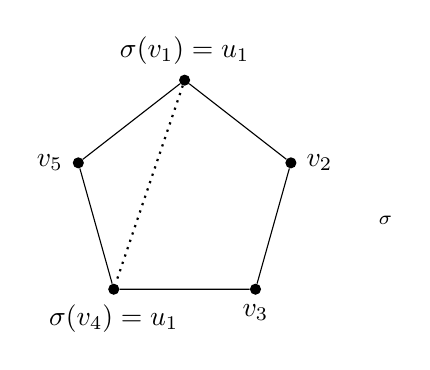
\begin{tikzpicture}[scale=1.5]
            \node[circle, fill, scale=0.015cm, label=above:{$\sigma(v_1)= u_1$}] (l1) at (0, 1) { };
            \node[circle, fill, scale=0.015cm, label=right:{$v_2$}] (l2) at (0.9, 0.30) { };
            \node[circle, fill, scale=0.015cm, label=below:{$v_3$}] (l3) at (0.6, -0.77) {};
            \node[circle, fill, scale=0.015cm, label=below:{$\sigma(v_4)=u_1$}] (l4) at (-0.6, -0.77) {};
            \node[circle, fill, scale=0.015cm, label=left:{$v_5$}] (l5) at (-0.9, 0.30) {};
            \draw (l1) -- (l2) -- (l3) -- (l4) -- (l5) -- (l1);
            \draw[dotted, thick] (l1) -- (l4);
            \node at (1.7, -0.2) { $\stackrel{\sigma}{\implies}$ };
        \end{tikzpicture}
        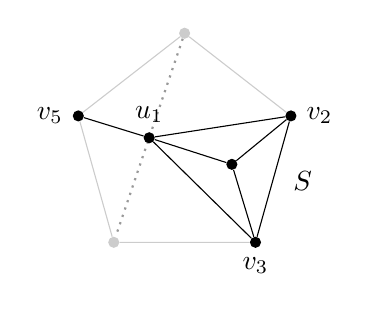
\begin{tikzpicture}[scale=1.5]
            \node[circle, fill, opacity=0.2, scale=0.015cm] (l1) at (0, 1) {};
            \node[circle, fill, opacity=0.2, scale=0.015cm] (l4) at (-0.6, -0.77) {};
            \node[circle, fill, scale=0.015cm, label=above:{$u_1$}] (y1) at (-0.3, 0.115) {};
    
            \node[circle, fill, scale=0.015cm, label=right:{$v_2$}] (l2) at (0.9, 0.30) { };
            \node[circle, fill, scale=0.015cm, label=below:{$v_3$}] (l3) at (0.6, -0.77) {};
            \node[circle, fill, scale=0.015cm, label=left:{$v_5$}] (l5) at (-0.9, 0.30) {};
    
            \node[circle, fill, scale=0.015cm] (s) at (0.4, -0.11) { };
            \node (s1) at (1.0, -0.25) { $S$ };
    
            \draw (s) -- (y1);
            \draw (s) -- (l3);
            \draw (s) -- (l2);

            \draw (l5) -- (y1) -- (l2) -- (l3) -- (y1);
            \draw[dotted, thick, opacity=0.4] (l1) -- (l4);
            \draw[opacity=0.2] (l5) -- (l1) -- (l2);
            \draw[opacity=0.2] (l3) -- (l4) -- (l5);
        \end{tikzpicture}
    \end{figure}
\end{frame}

\begin{frame}
    \frametitle{Reducers again}

    \begin{definition}
        A ring contraction $\sigma(v)$ on $R$ is a map from $R$ to the contracted ring $\sigma(R)$. Neighboring vertices of $R$ may not be mapped to the same vertex by $\sigma$.
    \end{definition}
    
    \begin{figure}[!h]
        \centering
        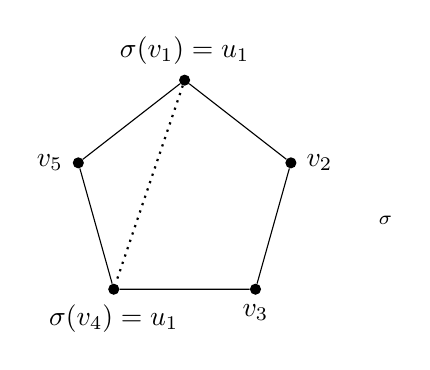
\begin{tikzpicture}[scale=1.5]
            \node[circle, fill, scale=0.015cm, label=above:{$\sigma(v_1)= u_1$}] (l1) at (0, 1) { };
            \node[circle, fill, scale=0.015cm, label=right:{$v_2$}] (l2) at (0.9, 0.30) { };
            \node[circle, fill, scale=0.015cm, label=below:{$v_3$}] (l3) at (0.6, -0.77) {};
            \node[circle, fill, scale=0.015cm, label=below:{$\sigma(v_4)=u_1$}] (l4) at (-0.6, -0.77) {};
            \node[circle, fill, scale=0.015cm, label=left:{$v_5$}] (l5) at (-0.9, 0.30) {};
            \draw (l1) -- (l2) -- (l3) -- (l4) -- (l5) -- (l1);
            \draw[dotted, thick] (l1) -- (l4);
            \node at (1.7, -0.2) { $\stackrel{\sigma}{\implies}$ };
        \end{tikzpicture}
        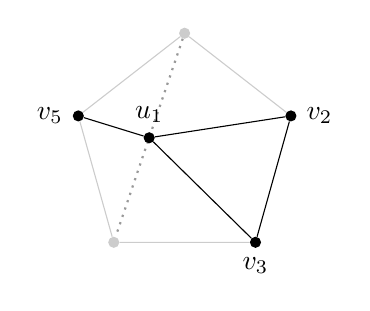
\begin{tikzpicture}[scale=1.5]
            \node[circle, fill, opacity=0.2, scale=0.015cm] (l1) at (0, 1) {};
            \node[circle, fill, opacity=0.2, scale=0.015cm] (l4) at (-0.6, -0.77) {};
            \node[circle, fill, scale=0.015cm, label=above:{$u_1$}] (y1) at (-0.3, 0.115) {};
    
            \node[circle, fill, scale=0.015cm, label=right:{$v_2$}] (l2) at (0.9, 0.30) { };
            \node[circle, fill, scale=0.015cm, label=below:{$v_3$}] (l3) at (0.6, -0.77) {};
            \node[circle, fill, scale=0.015cm, label=left:{$v_5$}] (l5) at (-0.9, 0.30) {};

            \draw (l5) -- (y1) -- (l2) -- (l3) -- (y1);
            \draw[dotted, thick, opacity=0.4] (l1) -- (l4);
            \draw[opacity=0.2] (l5) -- (l1) -- (l2);
            \draw[opacity=0.2] (l3) -- (l4) -- (l5);
        \end{tikzpicture}
    \end{figure}
    
\end{frame}

\begin{frame}
    \frametitle{Reducers again}

    \begin{definition}
        A reducer $(S,\sigma)$ of a configuration $\confg$ consists of
        \begin{itemize}
            \item A contraction $\sigma(v)$ on $R$.
            \item A graph $|S| < |\confg|$ whose boundary is the contracted ring $\sigma(R)$.
        \end{itemize}
    \end{definition}
    
    \begin{figure}[!h]
        \centering
        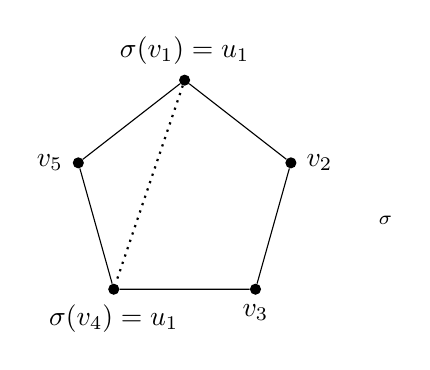
\begin{tikzpicture}[scale=1.5]
            \node[circle, fill, scale=0.015cm, label=above:{$\sigma(v_1)= u_1$}] (l1) at (0, 1) { };
            \node[circle, fill, scale=0.015cm, label=right:{$v_2$}] (l2) at (0.9, 0.30) { };
            \node[circle, fill, scale=0.015cm, label=below:{$v_3$}] (l3) at (0.6, -0.77) {};
            \node[circle, fill, scale=0.015cm, label=below:{$\sigma(v_4)=u_1$}] (l4) at (-0.6, -0.77) {};
            \node[circle, fill, scale=0.015cm, label=left:{$v_5$}] (l5) at (-0.9, 0.30) {};
            \draw (l1) -- (l2) -- (l3) -- (l4) -- (l5) -- (l1);
            \draw[dotted, thick] (l1) -- (l4);
            \node at (1.7, -0.2) { $\stackrel{\sigma}{\implies}$ };
        \end{tikzpicture}
        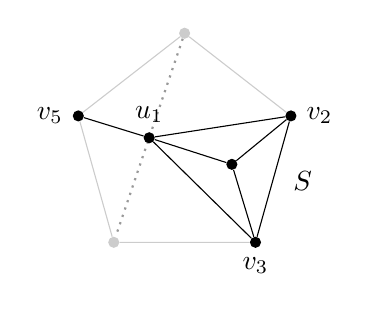
\begin{tikzpicture}[scale=1.5]
            \node[circle, fill, opacity=0.2, scale=0.015cm] (l1) at (0, 1) {};
            \node[circle, fill, opacity=0.2, scale=0.015cm] (l4) at (-0.6, -0.77) {};
            \node[circle, fill, scale=0.015cm, label=above:{$u_1$}] (y1) at (-0.3, 0.115) {};
    
            \node[circle, fill, scale=0.015cm, label=right:{$v_2$}] (l2) at (0.9, 0.30) { };
            \node[circle, fill, scale=0.015cm, label=below:{$v_3$}] (l3) at (0.6, -0.77) {};
            \node[circle, fill, scale=0.015cm, label=left:{$v_5$}] (l5) at (-0.9, 0.30) {};
            \node[circle, fill, scale=0.015cm] (s) at (0.4, -0.11) { };
            \node (s1) at (1.0, -0.25) { $S$ };
    
            \draw (s) -- (y1);
            \draw (s) -- (l3);
            \draw (s) -- (l2);
            \draw (l5) -- (y1) -- (l2) -- (l3) -- (y1);
            \draw[dotted, thick, opacity=0.4] (l1) -- (l4);
            \draw[opacity=0.2] (l5) -- (l1) -- (l2);
            \draw[opacity=0.2] (l3) -- (l4) -- (l5);
        \end{tikzpicture}
    \end{figure}
    
\end{frame}

\begin{frame}
    \frametitle{Reducer for the Bernhart Diamond}

    \begin{figure}[!h]
        \centering
        \begin{tikzpicture}[scale=1.5, mid arrow/.style={
            postaction={ decorate, decoration={ markings, mark=at position 0.6 with { \arrow[black]{>>} } } } }]
            \node[circle, fill, scale=0.015cm, label=left:$v_1$] (l1) at (-2, 0) { };
            \node[opacity=0.4] at (-1.2, 1.1) { $v_8$ };
            \node[circle, fill, scale=0.015cm, opacity=0.2] (l2) at (-1, 1) { };
            \node[opacity=0.4] at (-1.2, -1.1) { $v_2$ };
            \node[circle, fill, scale=0.015cm, opacity=0.2] (l4) at (-1, -1) {};
    
            \node[circle, fill, scale=0.015cm, label=right:$v_5$] (r1) at (2, 0) {};
            \node[opacity=0.4] at (1.2, 1.1) { $v_6$ };
            \node[circle, fill, scale=0.015cm, opacity=0.2] (r2) at (1, 1) {};
            \node[opacity=0.4] at (1.2, -1.1) { $v_4$ };
            \node[circle, fill, scale=0.015cm, opacity=0.2] (r4) at (1, -1) {};
    
            \node[circle, fill, scale=0.015cm, label=above:$v_7$] (b1) at (0, 1) {};
            \node[circle, fill, scale=0.015cm, label=below:$v_3$] (b2) at (0, -1) {};
            \node[circle, fill, scale=0.015cm, label=below left:$u_1$] (u1) at (0, 0.5) {};
            \node[circle, fill, scale=0.015cm, label=above left:$u_2$] (u2) at (0, -0.5) {};
    
            \draw[opacity=0.2] (l1) -- (l2) -- (b1) -- (r2) -- (r1) -- (r4) -- (b2) -- (l4);
            \draw [mid arrow, opacity=0.3] (l1) -- (l4);
            \draw (l1) -- (u1) -- (r1) -- (u2) -- (l1);
            \draw (b1) -- (u1);
            \draw (b2) -- (u2);
            \draw (u1) -- (u2);
            \draw[dotted, thick, opacity=0.4] (l2) -- (u1) -- (r2);
            \draw[dotted, thick, opacity=0.4] (l4) -- (u2) -- (r4);
    
        \end{tikzpicture}
    \end{figure}

    The reducer generates the following type of colorings.
    \begin{equation}
        v_1\;\colorbox{cyan}{$u_2$}\;v_3\;v_5\;\colorbox{magenta}{$u_1$}\;v_7 \quad \mapsto \quad v_1\;\colorbox{cyan}{$u_2$}\;v_3\;\colorbox{cyan}{$u_2$}\;v_5\;\colorbox{magenta}{$u_1$}\;v_7\;\colorbox{magenta}{$u_1$}.
    \end{equation}
\end{frame}

\begin{frame}
    \frametitle{C-reducibility}

    \begin{definition}
        A configuration $\confg$ is C-reducible if $\Phi(S,\sigma) \subset \overline{\Phi}(\confg)$ for some reducer $(S,\sigma)$.
    \end{definition}

    \begin{example}
        The Bernhart Diamond $(\ber)$ is C-reducible. The red colorings are \textit{symmetry faults} that can be shown to be fixable
    \end{example}
\end{frame}

\begin{frame}
    \frametitle{Symmetry Faults}

    The two red colorings generated by the reducer are not fixable. Does this mean that $\ber$ is not C-reducible?

    \begin{equation}
        \begin{aligned}
            \colorbox{rb}{abcbacbc} &\quad (R1) \\ \quad \colorbox{rb}{abcbdcbc} &\quad (R2)
        \end{aligned}
    \end{equation}

    \uncover<2->{
        Bernhart has shown in 1947 that these colorings \textit{can} in fact be fixed. So there must be an error in $\maxi{\ber}$.
    }
\end{frame}


\begin{frame}
    \frametitle{Symmetry Faults}

    Consider the following colorings.

    \begin{equation}
        \begin{aligned}
            \colorbox{rb}{abcbacbc} &\quad (R1) & \colorbox{sf}{\textcolor{white}{abcbadbc}} &\quad (F1) & \colorbox{rg}{\underline{abcbacac}} &\quad (G1)\\
             \quad \colorbox{rb}{abcbdcbc} &\quad (R2) & \quad \colorbox{g0}{abcbacbd} &\quad (F1\star) & \quad \colorbox{g0}{\underline{abcbdbcb}} &\quad (G2) \\
        \end{aligned}
    \end{equation}

    \uncover<2->{
    Then we have the implications

    \begin{equation}
        \begin{aligned}
        R2 \compat \{ G2, &R1 \} \\
        &\downarrow \\
        &R1 \compat \{ G1, F1 \} \\
        \end{aligned}
    \end{equation}

    Therefore, fixability of $R1$ and $R2$ depends fully on $F1$.
    }
\end{frame}

\begin{frame}
    \frametitle{Symmetry Faults}

    \begin{equation}
        \begin{aligned}
            \colorbox{rb}{abcbacbc} &\quad (R1) & \colorbox{sf}{\textcolor{white}{abcbadbc}} &\quad (F1) & \colorbox{rg}{\underline{abcbacac}} &\quad (G1)\\
             \quad \colorbox{rb}{abcbdcbc} &\quad (R2) & \quad \colorbox{g0}{abcbacbd} &\quad (F1\star) & \quad \colorbox{g0}{\underline{abcbdbcb}} &\quad (G2) \\
        \end{aligned}
    \end{equation}

    \begin{figure}[!h]
        \centering
        \begin{tikzpicture}[scale=1.5, mid arrow/.style={
            postaction={ decorate, decoration={ markings, mark=at position 0.6 with { \arrow[black]{>>} } } } }]
            \node (l1) at (-2, 0) { $a$ };
            \node (l2) at (-1, 1) { $c(d)$ };
            \node[circle, fill, scale=0.015cm, opacity=0.2] (l3) at (-1, 0) {};
            \node (l4) at (-1, -1) { $b$ };
    
            \node (r1) at (2, 0) { $a$ };
            \node (r2) at (1, 1) { $d(c)$ };
            \node[circle, fill, scale=0.015cm, opacity=0.2] (r3) at (1, 0) {};
            \node (r4) at (1, -1) { $b$ };
    
            \node[circle, fill, scale=0.015cm, opacity=0.2] (c1) at (0, 0.5) {};
            \node[circle, fill, scale=0.015cm, opacity=0.2] (c2) at (0, -0.5) {};
            \node (b1) at (0, 1) { $b$ };
            \node (b2) at (0, -1) { $c$ };
    
            \draw[thick, dotted] (0, -1.5) -- (0, 1.5);
            \draw[opacity=1.0] (l1) -- (l2) -- (b1) -- (r2) -- (r1) -- (r4) -- (b2) -- (l4);
            \draw[opacity=0.2] (c1) -- (b1);
            \draw[opacity=0.2] (c2) -- (b2);
    
            \draw [mid arrow, opacity=1.0] (l1) -- (l4);
            \draw[opacity=0.2] (l1) -- (l3);
            \draw[opacity=0.2] (l2) -- (l3) -- (l4);
            \draw[opacity=0.2] (l2) -- (c1);
            \draw[opacity=0.2] (c1) -- (l3) -- (c2);
            \draw[opacity=0.2] (c2) -- (l4);
            \draw[opacity=0.2] (c1) -- (c2);
            \draw[opacity=0.2] (r2) -- (c1);
            \draw[opacity=0.2] (c1) -- (r3) -- (c2);
            \draw[opacity=0.2] (c2) -- (r4);
            \draw[opacity=0.2] (r2) -- (r3) -- (r4);
            \draw[opacity=0.2] (r1) -- (r3);
        \end{tikzpicture}
    \end{figure}

    \uncover<2->{
        The colorings $F1$ and $F1\star$ are symmetric. Therefore, $F1$ must be fixable!
    }
\end{frame}

\begin{frame}
    \begin{definition}<1->
        A graph symmetry of $G$ is a bijection $f(v)$ on the vertices of $G$ that preserves the neighbors of every vertex.
    \end{definition}
    
    \begin{definition}<2->
        A \emph{symmetry fault} of a configuration $\confg$ is a coloring $x$ that is not in $\maxi{\confg}$, but whose symmetry $x\star = f(x)$ is.
    \end{definition}

    \uncover<3->{
        Bernhart mentioned the same problematic colorings in his proof. Is it a coincidence? We have not delved deeper into this problem.
    }
\end{frame}